\documentclass{beamer}
\usepackage[utf8]{inputenc}
\usepackage[T1]{fontenc}
% \usepackage{amscd, amsfonts, amsmath, amssymb, amstext, amsthm, caption, epsfig, fancyhdr, float, graphicx, latexsym, mathtools, multicol, multirow, algorithm, chngcntr}
\usepackage[english]{babel}
\usepackage{booktabs}

\usepackage{amsmath,amssymb}
\usepackage{graphicx}
\usepackage{caption}
\usepackage{subfig}
\usepackage{xspace}
\usepackage{fourier}

\usepackage{tikz}
\usetikzlibrary{shapes,arrows}
\usepackage{tkz-graph}
\usetikzlibrary{automata,arrows,positioning,calc}
\usetikzlibrary{positioning}
\usetikzlibrary{fit}
\usetikzlibrary{backgrounds}
\usetikzlibrary{calc}
\usetikzlibrary{shapes}
\usetikzlibrary{mindmap}
\usetikzlibrary{decorations.text}
\usetikzlibrary{snakes}

% \theoremstyle{definition} % insert bellow all blocks you want in normal text
% \newtheorem{definition}{Definition}



% tikzmark command, for shading over items
\newcommand{\tikzmark}[1]{\tikz[overlay,remember picture] \node (#1) {};}
% Define block styles
\tikzstyle{decision} = [diamond, draw, fill=blue!20,
    text width=4.5em, text badly centered, node distance=3cm, inner sep=0pt]
\tikzstyle{block} = [rectangle, draw, fill=blue!20,
    text width=5em, text centered, rounded corners]
\tikzstyle{line} = [draw]
\tikzstyle{cloud} = [draw, ellipse,fill=red!20, node distance=3cm,
    minimum height=2em]

\usepackage[most]{tcolorbox}

\setbeamertemplate{blocks}[rounded][shadow=true] % use rounded blocks with standard beamer shadow


% Distributions.
\newcommand*{\UnifDist}{\mathsf{Unif}}
\newcommand*{\ExpDist}{\mathsf{Exp}}
\newcommand*{\DepExpDist}{\mathsf{DepExp}}
\newcommand*{\GammaDist}{\mathsf{Gamma}}
\newcommand*{\LognormalDist}{\mathsf{LogNorm}}
\newcommand*{\WeibullDist}{\mathsf{Weib}}
\newcommand*{\ParetoDist}{\mathsf{Par}}
\newcommand*{\NormalDist}{\mathsf{Norm}}

\newcommand*{\GeometricDist}{\mathsf{Geom}}
\newcommand*{\NegBinomialDist}{\mathsf{NegBin}}
\newcommand*{\PoissonDist}{\mathsf{Poisson}}
\newcommand*{\BivariatePoissonDist}{\mathsf{BPoisson}}
\newcommand*{\CyclicalPoissonDist}{\mathsf{CPoisson}}

\newcommand*{\iid}{\textbf{iid}\@\xspace}
\newcommand*{\pdf}{\textbf{pdf}\@\xspace}
\newcommand*{\cdf}{\textbf{cdf}\@\xspace}
\newcommand*{\pmf}{\textbf{pmf}\@\xspace}
\newcommand*{\abc}{{\textbf{abc}}\@\xspace}
\newcommand*{\smc}{\textbf{smc}\@\xspace}
\newcommand*{\mcmc}{\textbf{mcmc}\@\xspace}
\newcommand*{\ess}{\textbf{ess}\@\xspace}
\newcommand*{\mle}{\textbf{mle}\@\xspace}
\newcommand*{\bic}{\textbf{bic}\@\xspace}
\newcommand*{\kde}{\textbf{kde}\@\xspace}
\newcommand*{\glm}{\textbf{glm}\@\xspace}
\newcommand*{\xol}{\textbf{xol}\@\xspace}
\newcommand*{\cpu}{\textbf{cpu}\@\xspace}
\newcommand*{\gpu}{\textbf{gpu}\@\xspace}
\newcommand*{\arm}{\textbf{arm}\@\xspace}

\def \si {\sigma}
\def \la {\lambda}
\def \al {\alpha}
% \def\e*{\end{eqnarray*}}
\def \di{\displaystyle}

\def \E{\mathbb E}
\def \N{\mathbb N}
\def \Z{\mathbb Z}
\def \NZ{\mathbb{N}_0}
\def \I{\mathbb I}
\def \w{\widehat}
\def \P {\mathbb P}
\def \V{\mathbb V}


\newcommand{\CL}{\mathbb{C}}
\newcommand{\RL}{\mathbb{R}}
\newcommand{\nat}{{\mathbb N}}
\newcommand{\Laplace}{\mathscr{L}}
\newcommand{\e}{\mathrm{e}}
\newcommand{\ve}{\bm{\mathrm{e}}} % vector e

\renewcommand{\L}{\mathcal{L}} % e.g. L^2 loss.

\newcommand{\ih}{\mathrm{i}}
\newcommand{\oh}{{\mathrm{o}}}
\newcommand{\Oh}{{\mathcal{O}}}
\newcommand{\Exp}{\mathbb{E}}

\newcommand{\Norm}{\mathcal{N}}
\newcommand{\LN}{\mathcal{LN}}
\newcommand{\SLN}{\mathcal{SLN}}

\renewcommand{\Pr}{\mathbb{P}}
\newcommand{\Ind}{\mathbb I}
\newcommand\bfsigma{\bm{\sigma}}
\newcommand\bfSigma{\bm{\Sigma}}
\newcommand\bfLambda{\bm{\Lambda}}
\newcommand{\stimes}{{\times}}
\def \limsup{\underset{n\rightarrow+\infty}{\overline{\lim}}}
\def \liminf{\underset{n\rightarrow+\infty}{\underline{\lim}}}




% vertical separator macro
\newcommand{\vsep}{
  \column{0.0\textwidth}
    
\begin{tikzpicture}
      \draw[very thick,black!10] (0,0) -- (0,7.3);
    \end{tikzpicture}
}
\newcommand\blfootnote[1]{%
  \begingroup
  \renewcommand\thefootnote{}\footnote{#1}%
  \addtocounter{footnote}{-1}%
  \endgroup
}

% More space between lines in align
% \setlength{\mathindent}{0pt}

% Beamer theme
\usetheme{ZMBZFMK}
\usefonttheme[onlysmall]{structurebold}
\mode<presentation>
\setbeamercovered{transparent=10}

% align spacing
\setlength{\jot}{0pt}

\setbeamertemplate{navigation symbols}{}%remove navigation symbols

\title[BLOCKASTICS]{Stochastic models for blockchain analysis}
\author{Pierre-O. Goffard}
\institute[UNISTRA]{Université de Strasbourg\\
 \texttt{goffard@unistra.fr}
}
\date{October 7, 2022}
% \titlegraphic{\includegraphics[width=2.5cm]{../../Figures/bfs_logo.png}} 

\begin{document}
\begin{frame}
  \titlepage
\end{frame}
\begin{frame}
  \tableofcontents
\end{frame}

% \section{Introduction}
\section{Blockchain}
\begin{frame}{Blockchain}
A decentralized data ledger made of blocks maintained by achieving consensus in a P2P network.
\begin{columns}
\begin{column}{0.5\textwidth}
% \small

\begin{itemize}
  \item Decentralized
  \item Public/private
  \item Permissionned/permissionless
  \item Immutable
  \item Incentive compatible
\end{itemize}
\end{column}
\begin{column}{0.5\textwidth}
\begin{center}
\begin{tikzpicture}[-, >=stealth', auto, semithick, node distance=01cm]
\tikzstyle{every edge}=[snake=expanding waves,segment length=1mm,segment angle=10, draw]

\tikzstyle{full node}=[circle, fill=tublue,draw=tublue,thick,text=black,scale=0.8]
\tikzstyle{light node}=[circle, fill=white,draw=tublue,thick,text=black,scale=0.8]
\node[full node]    (1)                     {};
\node[full node]    (2)[above right of=1]         {};
\node[full node]    (3)[above left of=1]         {};
\node[full node]    (4)[below of=1]         {};
\node[full node]    (5)[right of=4]         {};
\node[full node]    (6)[below of=4]         {};
\node[light node]    (7)[left of=1]         {};
\node[light node]    (8)[right of=2]         {};
\node[light node]    (9)[left of=4]         {};
\node[light node]    (10)[above right of=5]         {};
\node[light node]    (11)[ right of=5]         {};
\node[light node]    (12)[ below right of=5]         {};
% \node[light node]    (4)[above of=2]         {};
\path

(1) edge node{} (2)
    edge node{} (3)
    edge node{} (7)
    ;
\path
(5) edge node{} (10)
    edge node{} (11)
    edge node{} (12)
    ;
    \path
(4) edge node{} (5)
    edge node{} (1)
    edge node{} (9)
    edge node{} (6)
    ;
    \path
(2) edge node{} (8)   
    ;
\end{tikzpicture}
\end{center}
\end{column}
\end{columns}

\vspace{0.2cm}
 
\end{frame}
\begin{frame}{Applications of blockchain: Cryptocurrency}
\begin{columns}
\begin{column}{0.5\textwidth}
   
{\footnotesize
\begin{thebibliography}{1}
\bibitem{Na08}
S.~Nakamoto, ``Bitcoin: A peer-to-peer electronic cash system.'' Available at
  \href{https://bitcoin.org/bitcoin.pdf}{https://bitcoin.org/bitcoin.pdf},
  2008.
\end{thebibliography}  
}
\end{column}
\begin{column}{0.5\textwidth}  %%<--- here
    \begin{center}
     
\includegraphics[width=0.5\textwidth]{../../Figures/bitcoin-6284869_1920.png}
     \end{center}
\end{column}
\end{columns}

\begin{itemize}
  \item Transaction anonymity
  \item Banking and reliable currency in certain regions of the world
  \item Money Transfer worldwide (at low fare)
  \item No need for a thrusted third party
  \item Proof of Work (\textbf{PoW})
\end{itemize}
\end{frame}

\begin{frame}{Consensus protocols}
The mechanism to make all the nodes agree on a common data history using the network ressources
\vspace{0.3cm}
\begin{itemize}
  \item Bandwidth
  \item Storage
  \item Computing power
  \item Cryptocurrency
\end{itemize}
\end{frame}
\begin{frame}{Consensus protocols}
The three dimensions of blockchain systems analysis
\begin{enumerate}
  \item Efficiency (Queueing model)
  \begin{itemize}
    \item Throughputs
    \item Transaction confirmation time
  \end{itemize}
    \item Security (Insurance risk model)
  \begin{itemize}
    \item Resistance to attacks
  \end{itemize}
  \item Decentralization (stochastic processes with reinforcement)
  \begin{itemize}
    \item Fair distribution of the accounting right
  \end{itemize}

\end{enumerate}
\begin{tcolorbox}[enhanced,drop shadow, title=BLOCKASTICS project]
Analysis and optimization of blockchain systems.
\end{tcolorbox}
\blfootnote{ 
\href{https://pierre-olivier.goffard.me/BLOCKASTICS/}{\texttt{link}}}
\end{frame}
\begin{frame}{Blockchain as a research topic}

\begin{itemize}
  \item Computer science
  \begin{itemize}
  \item Peer-to-peer networks and consensus algorithm
  \item Cryptography and security
  \end{itemize}
  \item Economics  
  \begin{itemize}
  \item Game theory to study the incentive mechanism at play
  \item Nature of the cryptoassets
  \end{itemize}
  \item Operations research  
  \begin{itemize}
  \item Optimization of complex system
  \end{itemize}
  \item Financial math  
  \begin{itemize}
  \item Valuation models for cryptoassets
  \end{itemize}
  \item Machine learning and statistics  
  \begin{itemize}
  \item Open data
  \item Interaction between blockchain users
  \item (Social) network analysis
  \item Clustering of public keys and addresses in the bitcoin blockchain.
  \end{itemize}
\end{itemize}
\end{frame}
\begin{frame}{My contributions}
\begin{itemize}
\item Security of \textbf{PoW} blockchains
\tiny
\begin{thebibliography}{1}

\bibitem{Hansjoerg2022}
Hansjoerg Albrecher and Pierre-Olivier Goffard.
\newblock On the profitability of selfish blockchain mining under consideration
  of ruin.
\newblock {\em Operations Research}, 70(1):179--200, jan 2022.


\bibitem{Goffard2019}
Pierre-O. Goffard.
\newblock Fraud risk assessment within blockchain transactions.
\newblock {\em Advances in Applied Probability}, 51(2):443--467, jun 2019.
\newblock \url{https://hal.archives-ouvertes.fr/hal-01716687v2}.

\end{thebibliography}
\normalsize
\item  Decentralization of \textbf{PoW} blockchains
\tiny
\begin{thebibliography}{1}
\bibitem{Albrecher2022}
Hansjörg Albrecher, Dina Finger, and Pierre-O. Goffard.
\newblock Blockchain mining in pools: Analyzing the trade-off between
  profitability and ruin.
\newblock {\em Insurance: Mathematics and Economics}, 105:313--335, jul 2022.
\end{thebibliography}
\end{itemize}
\end{frame}
\section{Insurance risk theory}
\begin{frame}{Cramer-Lunberg model}
\begin{columns}
\begin{column}{0.5\textwidth}
\scriptsize
The financial reserves of an insurance company over time have the following dynamic
\begin{equation*}
R_t = z +ct - \sum_{i = 1}^{N_t}U_i\text{, }t\geq0,
\end{equation*}
where 
\begin{itemize}
  \item $z>0$ denotes the initial reserves
  \item $c$ is the premium rate
  \item $(N_t)_{t\geq0}$ is a counting process that models the claim arrival 
  \begin{itemize}
    \scriptsize
    \item[$\hookrightarrow$]  Poisson process with intensity $\lambda$
  \end{itemize}
  \item The $U_i$'s are the randomly sized compensations
  \begin{itemize}
    \scriptsize
    \item[$\hookrightarrow$] non-negative, \textbf{i.i.d.}
  \end{itemize}
\end{itemize}
\end{column}
\begin{column}{0.5\textwidth}
\begin{tikzpicture}
  %Origin and axis
  \coordinate (O) at (0,0);
  \draw[->] (-0.5,0) -- (5.5,0) coordinate[label = {below:\scriptsize$t$}] (xmax);
  \draw[->] (0,-0.5) -- (0,4) coordinate[label = {right:\scriptsize$R_t$}] (ymax);
   %Initial reserves
  \draw (0,2) node[black,left] {\scriptsize$z$} node{};
 % % %Length of the honest chain
  \draw[thick, tublue,-] (0,2) -- (2,3) node[pos=0.5, above] {};
  \draw[thick, dashed, tublue] (2,3) -- (2,1) node[pos=0.5, left] {\scriptsize\color{black}$U_1$};
  \draw[thick, tublue] (2,1) -- (3,1.5) node[pos=0.5, above] {};
  \draw[thick, dashed, tublue] (3,1.5) -- (3, 0.5) node[pos=0.5, left] {\scriptsize\color{black}$U_2$};
  \draw[thick, tublue] (3,0.5) -- (5, 1.5) node[pos=0.5, above] {};
   \draw[thick, dashed, tublue] (5,1.5) -- (5, -0.5) node[pos=0.5,above left] {\scriptsize\color{black}$U_3$};

  %Block finding Times 
  \draw (2,0) node[black,below] {\scriptsize$T_1$} node{ \color{black}$\bullet$};
  \draw (3,0) node[black,below] {\scriptsize$T_2$} node{ \color{black}$\bullet$};
  \draw (5,0) node[black,below left] {\scriptsize$\tau_z$} node{ \color{black}$\bullet$};
\end{tikzpicture}
\end{column}
\end{columns}

\end{frame}
\begin{frame}{Ruin probabilities}
\scriptsize
Define the ruin time as 
$$
\tau_z = \inf\{t\geq0\text{ ; }R_t <0\}
$$
and the ruin probabilities as 
$$
\psi(z,t) = \mathbb{P}(\tau_z < t)\text{ and }\psi(z) = \mathbb{P}(\tau_z < \infty)
$$
We look for $z$ such that 
$$
\mathbb{P}(\text{Ruin}) = \alpha\text{ (0.05)},
$$
given that 
$$
c=(1+\eta)\lambda\mathbb{E}(U),
$$
with 
$$\eta>0\text{ (net profit condition)}$$  
otherwise 
$$\psi(z)=1.$$

\tiny
\begin{thebibliography}{1}

\bibitem{Asmussen_2010}
S.~Asmussen and H.~Albrecher, {\em Ruin Probabilities}.
\newblock {WORLD} {SCIENTIFIC}, sep 2010.

\end{thebibliography}

\end{frame}
\begin{frame}{My contributions}
Numerical approximations via Laplace transform inversion 
\tiny
\begin{thebibliography}{1}

\bibitem{Asmussen2019}
S{\o}ren Asmussen, Pierre-Olivier Goffard, and Patrick~J. Laub.
\newblock Orthonormal polynomial expansions and lognormal sum densities.
\newblock In {\em Risk and Stochastics}, pages 127--150. {WORLD} {SCIENTIFIC}
  ({EUROPE}), apr 2019.

\bibitem{Goffard2020}
Pierre-Olivier Goffard and Patrick~J. Laub.
\newblock Orthogonal polynomial expansions to evaluate stop-loss premiums.
\newblock {\em Journal of Computational and Applied Mathematics}, 370:112648,
  may 2020.

\bibitem{Goffard2015}
Pierre-Olivier Goffard, St{\'{e}}phane Loisel, and Denys Pommeret.
\newblock Polynomial approximations for bivariate aggregate claims amount
  probability distributions.
\newblock {\em Methodology and Computing in Applied Probability},
  19(1):151--174, nov 2015.

\bibitem{Goffard2016}
Pierre-Olivier Goffard, St{\'{e}}phane Loisel, and Denys Pommeret.
\newblock A polynomial expansion to approximate the ultimate ruin probability
  in the compound poisson ruin model.
\newblock {\em Journal of Computational and Applied Mathematics}, 296:499--511,
  apr 2016.

\end{thebibliography}


\end{frame}
\begin{frame}{My contributions}
Closed form expressions via combinatorial analysis 
\tiny
\begin{thebibliography}{1}

\bibitem{Goffard2017a}
Pierre-Olivier Goffard.
\newblock Two-sided exit problems in the ordered risk model.
\newblock {\em Methodology and Computing in Applied Probability},
  21(2):539--549, nov 2017.

\bibitem{Goffard2017}
Pierre-Olivier Goffard and Claude Lef{\`{e}}vre.
\newblock Boundary crossing of order statistics point processes.
\newblock {\em Journal of Mathematical Analysis and Applications},
  447(2):890--907, mar 2017.

\bibitem{Goffard2018}
Pierre-Olivier Goffard and Claude Lef{\`{e}}vre.
\newblock Duality in ruin problems for ordered risk models.
\newblock {\em Insurance: Mathematics and Economics}, 78:44--52, jan 2018.

\end{thebibliography}

\end{frame}
\section{Applications of Bayesian statistics in actuarial science}
\begin{frame}{Bayesian statistics}
\small
Let $\mathcal{M}$ be a model with parameters $\mathbf{\theta}$, and $\mathbf{x}$ some observed data. 
\begin{itemize}
\item Bayesian statistics targets the posterior distribution of the parameters 
\begin{equation*}
\pi(\mathbf{\theta}|\mathbf{x}) = \frac{p(\mathbf{x}|\theta)\pi(\mathbf{\theta})}{\int_{\Theta}p(\mathbf{x}|\theta)\pi(\mathbf{\theta})\text{d}\mathbf{\theta}} =  \frac{p(\mathbf{x}|\theta)\pi(\mathbf{\theta})}{Z(\mathbf{x})},
\end{equation*}
by updating the prior $\pi(\mathbf{\theta})$ via the likelihood $p(\mathbf{x}|\theta)$.
\item[\tiny$\hookrightarrow$] Model calibration
\end{itemize}
If many models $\mathcal{M}_1,\ldots,  \mathcal{M}_K$ are competing  
\begin{itemize}
\item The posterior model evidence of each model follow from 
\begin{equation*}
\pi(M_i|\mathbf{x}) = \frac{p(\mathbf{x}|M_i)\pi(\mathcal{M}_i)}{\sum_{j = 1}^Kp(\mathbf{x}|M_j)\pi(\mathcal{M}_j)},\text{ }i=1,\ldots, K.
\end{equation*}
\item[$\hookrightarrow$] Select or combine models 
\end{itemize}
\end{frame}
\begin{frame}{My contributions}
\begin{itemize}
  \item Mortality forecasting using demographic projection model and STAN 
  \tiny
  \begin{thebibliography}{1}

\bibitem{Barigou2022}
Karim Barigou, Pierre-Olivier Goffard, St{\'{e}}phane Loisel, and Yahia Salhi.
\newblock Bayesian model averaging for mortality forecasting using
  leave-future-out validation.
\newblock {\em International Journal of Forecasting}, mar 2022.
\end{thebibliography}
 \normalsize
\item Sequential Monte Carlo Sampler to fit composite models
  \tiny
  \begin{thebibliography}{1}
\bibitem{goffard:hal-03263471}
Pierre-Olivier Goffard.
\newblock {Sequential Monte Carlo samplers to fit and compare insurance loss
  models}.
\newblock working paper or preprint, March 2022.
\end{thebibliography}
 \normalsize
\item Approximate Bayesian Computation with aggregated data
\tiny
\begin{thebibliography}{1}
\bibitem{Goffard2021}
Pierre-Olivier Goffard and Patrick~J. Laub.
\newblock Approximate bayesian computations to fit and compare insurance loss
  models.
\newblock {\em Insurance: Mathematics and Economics}, 100:350--371, sep 2021.

\end{thebibliography}

\end{itemize}

\end{frame}
{ % all template changes are local to this group.
    \setbeamertemplate{navigation symbols}{}
    \begin{frame}[plain]
        \begin{tikzpicture}[remember picture,overlay]
            \node[at=(current page.center)] {
                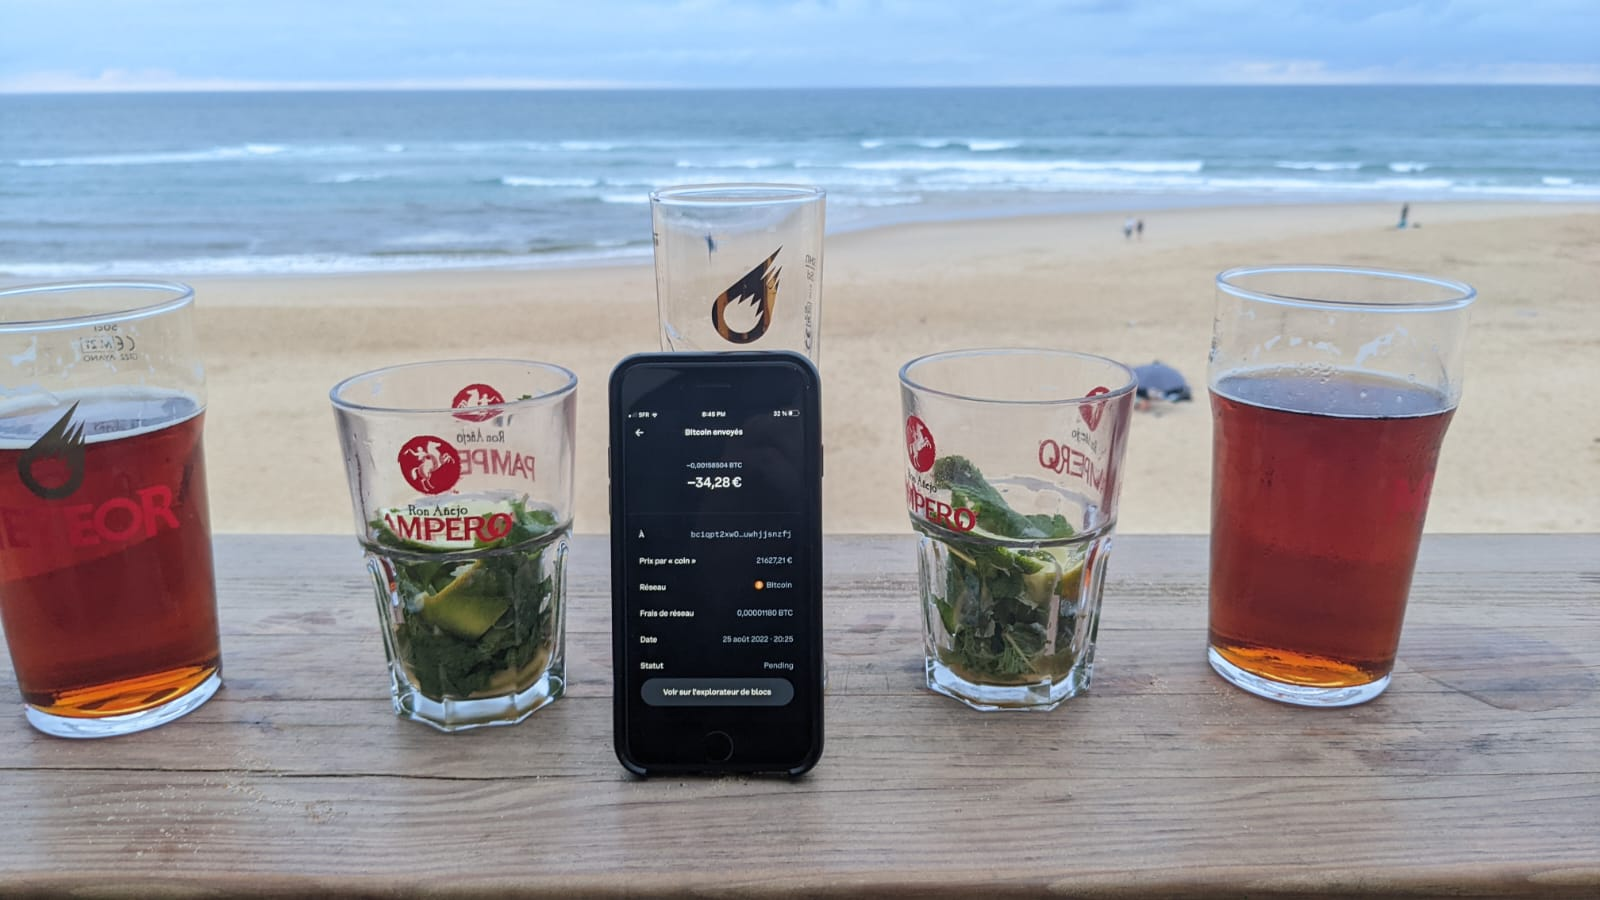
\includegraphics[width=\textwidth]{../../Figures/bitcoin_cocktail.jpg}
            };
        \end{tikzpicture}
     \end{frame}
}

% \begin{frame}{Decentralized finance}
% DEFI creates new financial architecture
% \begin{columns}
% \begin{column}{0.5\textwidth}
% \begin{itemize}
% \item[+] Non custodial
% \item[+] Anonymous
% \item[+] Permisionless
% \item[+] openly auditable
% \end{itemize}
% \end{column}
% \begin{column}{0.5\textwidth} 
% \begin{itemize}
% \item[-] Unregulated
% \item[-] Tax evasion
% \item[-] Fraud
% \item[-] Money laundering
% \end{itemize} 
% \end{column}
% \end{columns}
% \vspace{0.5cm}
% Extends the Bitcoin promises to more complex financial operations
% \begin{itemize}
%   \item Collateralized lending
%   \item Decentralized Exchange Platform
%   \item Tokenized assets
%   \item Fundraising vehicle (ICO, STO, ...)
% \end{itemize}
% \vspace{0.3cm}
% \scriptsize
% \begin{thebibliography}{1}

% \bibitem{werner2021sok}
% S.~M. Werner, D.~Perez, L.~Gudgeon, A.~Klages-Mundt, D.~Harz, and W.~J.
%   Knottenbelt, ``Sok: Decentralized finance (defi),'' 2021.

% \end{thebibliography}

% \end{frame}
\appendix
\begin{frame}{What's inside a block?}
A block consists of 
\begin{itemize}
\item a header 
\item a list of "transactions" that represents the information recorded through the blockchain. 
\end{itemize}
The header usually includes 
\begin{itemize}
\item the date and time of creation of the block, 
\item the block height which is the index inside the blockchain, 
\item the hash of the block 
\item the hash of the previous block. 
\end{itemize}
\begin{tcolorbox}[enhanced,drop shadow, title=Question]
What is the hash of a block?
\end{tcolorbox}
\end{frame}
\begin{frame}{Cryptographic Hash function}
\small
A function that maps data of arbitratry size (message) to a bit array of fixed size (hash value)
$$
h:\{0,1\}^\ast\mapsto \{0,1\}^d. 
$$
A good hash function is
\begin{itemize}
\item deterministic
\item quick to compute
\item One way
\begin{itemize}
  \scriptsize
\item[$\hookrightarrow$] For a given hash value $\overline{h}$ it is hard to find a message $m$ such that 
$$
h(m) = \overline{h}
$$
\end{itemize}
\item Colision resistant 
\begin{itemize}
\item[$\hookrightarrow$] Impossible to find $m_1$ and $m_2$ such that 
$$
h(m_1) = h(m_2)
$$
\end{itemize}
\item Chaotic
$$m_1\approx m_2\Rightarrow  h(m_1) \neq h(m_2)$$
\end{itemize}
\end{frame}
\begin{frame}{SHA-256}
The SHA-256 function which converts any message into a hash value of $256$ bits.
\begin{tcolorbox}[enhanced,drop shadow, title=Example]
The hexadecimal digest of the message
$$
\texttt{Bienvenue à l'IRMA}
$$
is 
\footnotesize
$$
\texttt{50f3257a3d22a56247a8978fd2505e8cdd64e1cb06e52c941d09e234722dc275}
$$
\end{tcolorbox}
\end{frame}
\begin{frame}{Mining a block}
\begin{figure}[!ht]
    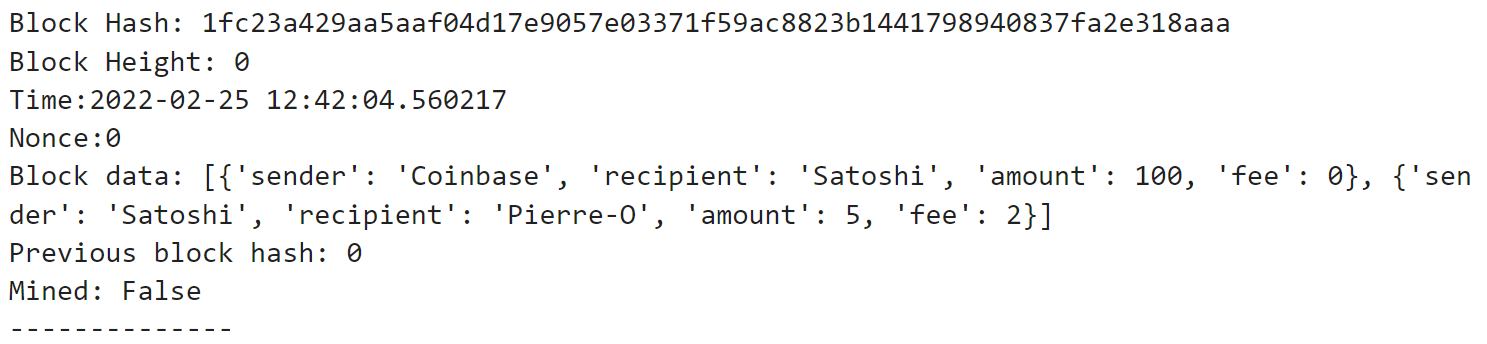
\includegraphics[width = \textwidth]{../../Figures/block_not_mined.png}
    \captionsetup{width=0.8\textwidth}
    \centering
    \caption{A block that has not been mined yet.}
    \label{fig:block_not_mined}
\end{figure}
\end{frame}
\begin{frame}{Mining a block}
The maximum value for a 256 bits number is
$$
T_\text{max} = 2^{256}-1 \approx 1.16e^{77}.
$$
Mining consists in drawing at random a nonce 
$$
\text{Nonce} \sim \text{Unif}(\{0,\ldots, 2^{32}-1\}),
$$
until 
$$
h(\text{Nonce}|\text{Block info})<T,
$$
where $T$ is referred to as the target.
\begin{tcolorbox}[enhanced,drop shadow, title=Difficulty of the cryptopuzzle]
$$
D = \frac{T_{\max}}{T}.
$$
\end{tcolorbox}

\end{frame}
\begin{frame}{Mining a block}
If we set the difficulty to $D = 2^4$ then the hexadecimal digest must start with at least $1$ leading $0$
\begin{figure}[!ht]
    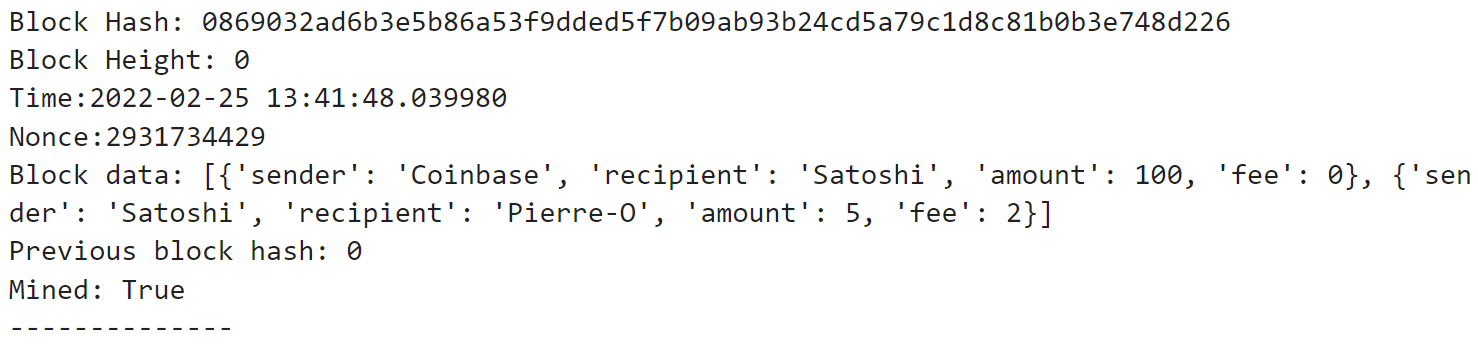
\includegraphics[width = \textwidth]{../../Figures/block_mined.png}
    \captionsetup{width=0.8\textwidth}
    \centering
    \caption{A mined block with a hash value having on leading zero.}
    \label{fig:block_mined}
\end{figure}
The number of trial is geometrically distributed
\begin{itemize}
\item Exponential inter-block times
\item Lenght of the blockchain = Poisson process
\end{itemize}
\end{frame}
\begin{frame}{Bitcoin protocol}
\begin{itemize}
  \item One block every 10 minutes on average
  \item Depends on the hashrate of the network
  \item Difficulty adjustment every 2,016 blocks ($\approx$ two weeks)
  \item Reward halving every 210,000 blocks
\end{itemize}
Check out \url{https://www.bitcoinblockhalf.com/}
\end{frame}
\section{Blockchain efficiency}
\begin{frame}{Efficiency}
Efficiency is characterized by 
\begin{itemize}
  \item Throughputs: Number of transaction being processed per time unit
  \item Latency: Average transaction confirmation time
\end{itemize}

\end{frame}
\begin{frame}{Queue settings}
\begin{center}
\begin{tikzpicture}[-, >=stealth', auto, semithick, node distance=1cm]

\tikzstyle{phantom block}=[rectangle, fill=white,draw=white, thick,text=black,scale=2]
\tikzstyle{block}=[rectangle, fill=white,draw=black,thick,text=black,scale=4]
\tikzstyle{Intensity}=[circle, fill=white,draw=tublue,very thick, text=black,scale=1.2]
\tikzstyle{transaction pending}=[circle, fill=white,draw=tublue,very thick, text=black,scale=1]
\tikzstyle{transaction considered}=[circle, fill=tublue, text=black, scale=1]
\node[Intensity]    (1){$\lambda$};
\node[phantom block]  (2)[right of=1] {};
\node[transaction pending] (3)[right of=2] {};
\node[transaction pending] (4)[above of=3] {};
\node[transaction pending] (5)[above of=4] {};
\node[transaction pending] (6)[above of=5] {};
\node[transaction pending] (7)[below of=3] {};
\node[transaction pending] (8)[below of=7] {};
\path
(1) edge[->,bend left]     node{} (4)
    edge[->, bend right]     node{}          (7);
\pause
\node[Intensity]  (14)[above of=6]{$\mu$};
% \path
% (1) edge[->,bend left]     node{$\text{Exp}(\lambda)$}        (4)
%     edge[->, bend right]     node{}          (7);
\pause
\node[transaction considered] (3)[right of=2] {};
\node[transaction considered] (4)[above of=3] {};
\node[transaction considered] (5)[above of=4] {};
\node[transaction considered] (6)[above of=5] {};

\pause
\node[phantom block]  (10)[right of=3] {};
\node[block]  (11)[right of=10] {};
\path
(6) edge[->]   node{} (11)
(5) edge[->]   node{} (11)
(4) edge[->]   node{} (11)
(3) edge[->]   node{} (11)
;
\node[Intensity]  (12)[above of=11] {$\mu$};
\node[phantom block]  (13)[above of=12] {};

\path
(11) edge[-]     node{}        (12);
\path
(12) edge[->]     node{}        (13);

\end{tikzpicture}
\end{center}
\end{frame}
\begin{frame}{Queueing setting}
\begin{itemize}
\item Poisson arrival with rate $\lambda>0$ for the transactions
\item Poisson arrival with rate $\mu>0$ for the blocks 
\item Block size $b\in\mathbb{N}^\ast$
$\Rightarrow $Batch service
\item[\warning] The server is always busy
\end{itemize}
This is somekind of $M/M^b/1$ queue.
\tiny
\begin{thebibliography}{1}
\bibitem{Kawase2017}
Y.~Kawase and S.~Kasahara, ``Transaction-confirmation time for bitcoin:
  A~queueing analytical approach to~blockchain~mechanism,'' in {\em Queueing
  Theory and Network Applications}, pp.~75--88, Springer International
  Publishing, 2017.
\bibitem{Bailey1954}
N.~T.~J. Bailey, ``On queueing processes with bulk service,'' {\em Journal of
  the Royal Statistical Society: Series B (Methodological)}, vol.~16,
  pp.~80--87, jan 1954.

\bibitem{Cox1955}
D.~R. Cox, ``The analysis of non-markovian stochastic processes by the
  inclusion of supplementary variables,'' {\em Mathematical Proceedings of the
  Cambridge Philosophical Society}, vol.~51, pp.~433--441, jul 1955.

\end{thebibliography}
\end{frame}
\section{Blockchain security}
\begin{frame}{Double spending attack}
\scriptsize
\begin{enumerate}
\item Mary transfers 10 BTCs to John
\item The transaction is recorded in the public branch of the blockchain and John ships the good.
\item Mary transfers to herself the exact same BTCs
\item The malicious transaction is recorded into a private branch of the blockchain
\begin{itemize}
  \scriptsize
\item Mary has friends among the miners to help her out
\item The two chains are copycat up to the one transaction
\end{itemize}
\end{enumerate}
\begin{tcolorbox}[enhanced,drop shadow, title=Fact (Bitcoin has only one rule)]
The longest chain is to be trusted
\end{tcolorbox}
\end{frame}
\begin{frame}{Double spending in practice}
\scriptsize
Vendor are advised to wait for $\alpha\in\mathbb{N}$ of confirmations so that the honest chain is ahead of the dishonest one.
\begin{center}
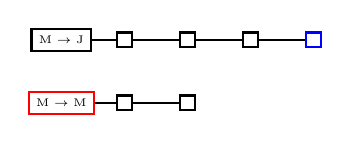
\begin{tikzpicture}[-, >=stealth', auto, semithick, node distance=1cm]
% \tikzstyle{block} = [rectangle, draw, fill=blue!20,
%     text width=5em, text centered, rounded corners]
\tikzstyle{block}=[rectangle, fill=black,draw=black,thick,text=black,scale=0.6]
\tikzstyle{block}=[rectangle, fill=white,draw=black,thick,text=black,scale=0.8]
\tikzstyle{confirmed block}=[rectangle, fill=white,draw=blue,thick,text=black,scale=0.8]
\tikzstyle{bad block}=[rectangle, fill=white,draw=red,thick,text=black,scale=0.8]
\node[block]    (1)                     {\tiny $\text{M}\rightarrow \text{J}$};
\node[block]    (2)[right of=1]                     {};
\node[block]    (3)[right of=2]                     {};
\node[block]    (4)[right of=3]                     {};
\node[confirmed block]    (5)[right of=4]                     {};

\node[bad block]    (6)[below of=1]         {\tiny $\text{M}\rightarrow \text{M}$};
\node[block]    (7)[right of=6]         {};
\node[block]    (8)[right of=7]         {};
\path
(1) edge[ left]     node{}     (2)
(2) edge[ left]     node{}     (3)
(3) edge[ left]     node{}     (4)
(4) edge[ left]     node{}     (5)
(6) edge[ left]     node{}     (7)
(7) edge[ left]     node{}     (8);

\end{tikzpicture}
\end{center}
In the example, vendor awaits $\alpha = 4$ confirmations, the honest chain is ahead of the dishonest one by $z = 2$ blocks.
\begin{tcolorbox}[enhanced,drop shadow, title=Fact (PoW is resistant to double spending)]
\begin{itemize}
\item Attacker does not own the majority of computing power 
\item Suitable $\alpha$ 
\end{itemize}
Double spending is unlikely to succeed.
\end{tcolorbox}
\tiny
\begin{thebibliography}{1}
\bibitem{Na08}
S.~Nakamoto, ``Bitcoin: A peer-to-peer electronic cash system.'' Available at
  \href{https://bitcoin.org/bitcoin.pdf}{https://bitcoin.org/bitcoin.pdf},
  2008.
  
\end{thebibliography}

\end{frame}
\begin{frame}{Mathematical set up}
\begin{columns}
\begin{column}{0.5\textwidth}
\scriptsize

Let the length of honest and dishonest chain be driven by counting processes
\begin{itemize}
\item Honest chain $\Rightarrow$ $z+N_t\text{ , }t\geq0$, where $z\geq1$.
\item Malicious chain $\Rightarrow$ $M_t\text{ , }t\geq0$
\item Study the distribution of the first-\textit{rendez-vous} time
$$
\tau_z=\inf\{t\geq0\text{ , } M_t=z+N_t\}.
$$
\end{itemize}
If $N_t\sim\text{Pois}(\lambda t)$ and $M_t\sim\text{Pois}(\mu t)$ such that $\lambda>\mu$ then 
$$
\mathbb{P}(\tau_z <\infty) = \left(\frac{\mu}{\lambda}\right)^z,\text{ }z\geq 0.
$$
\end{column}
\begin{column}{0.5\textwidth}
\begin{tikzpicture}
  %Origin and axis
  \coordinate (O) at (0,0);
  \draw[->] (-0.5,0) -- (5.5,0) coordinate[label = {above:\scriptsize$t$}] (xmax);
  \draw[->] (0,-0.5) -- (0,5) coordinate[label = {right:\scriptsize$n$}] (ymax);
 %Length of the honest chain
  \draw[thick,tublue,-] (0,3) -- (2,3) node[pos=0.5, above] {} ;
  \draw[thick,tublue] (2,3) -- (2,4) node[pos=0.5, above] {};
  \draw[thick,tublue] (2,4) -- (5.5,4) node[pos=0.5, right] {};
  % %Length of the Malicious chain
  \draw[very thick,dashed,red,-] (0,0) -- (0.75,0) node[pos=0.5, above] {} ;
  \draw[very thick,dashed,red] (0.75,0) -- (0.75,1) node[pos=0.5, right] {};
  \draw[very thick,dashed,red] (0.75,1) -- (1.25,1) node[pos=0.5, above] {};
  \draw[very thick,dashed,red] (1.25,1) -- (1.25,2) node[pos=0.5, right] {};
  \draw[very thick,dashed,red] (1.25,2) -- (2.5,2) node[pos=0.5, above] {};
  \draw[very thick,dashed,red] (2.5,2) -- (2.5,3) node[pos=0.5, right] {};
  \draw[very thick,dashed,red] (2.5,3) -- (5,3) node[pos=0.5, right] {};
  \draw[very thick,dashed,red] (5,3) -- (5,4) node[pos=0.5, above] {};
  \draw[very thick,dashed,red] (5,4) -- (5.5,4) node[pos=0.5, above] {};
  %Jump Times of the malicious chain
  \draw (0.75,0) node[red,below] {\scriptsize$S_1$} node{ \color{red}$\bullet$};
  \draw (1.25,0) node[red,below] {\scriptsize$S_2$} node{ \color{red}$\bullet$};
  \draw (2.5,0) node[red,below] {\scriptsize$S_3$} node{ \color{red}$\bullet$};
  \draw (5,0) node[black,below] {\scriptsize$S_4=\tau_z$} node{ \color{black}$\bullet$};
  % %Jump Times of the honest chain
  \draw (2,0) node[tublue,below] {\scriptsize$T_1$} node{ \color{tublue}$\bullet$};
  % %Aggregated Capital gains
  \draw (0,1) node[black,left] {\scriptsize$1$} node{ \color{black}$-$};
  \draw (0,2) node[black,left] {\scriptsize$2$} node{ \color{black}$-$};
  \draw (0,3) node[black,left] {\scriptsize$z$} node{};
  \draw (0,4) node[black,left] {\scriptsize$4$} node{ \color{black}$-$};
  % %Ruin time = First-meeting time
  % \draw (7,0) node[black,below] {$\tau_z$} node{ \color{black}$\times$};
  % \draw[dotted,black] (7,3) -- (7,0);
\end{tikzpicture}
\end{column}
\end{columns}

\tiny
\begin{thebibliography}{1}

\bibitem{Goffard2019}
P.-O. Goffard, ``Fraud risk assessment within blockchain transactions,'' {\em
  Advances in Applied Probability}, vol.~51, pp.~443--467, jun 2019.
\newblock \url{https://hal.archives-ouvertes.fr/hal-01716687v2}.

\end{thebibliography}

\end{frame}
\section{Blockchain Decentralization}
\begin{frame}{Proof of Stake protocol}
\scriptsize
PoS is the most popular alternative to PoW.
\begin{itemize}
  \item A block validator is selected according to the number of native coins she owns
  \item Update the blockchain and receive a reward or do nothing  
\end{itemize}
Two problems 
\begin{itemize}
  \item[\warning] Nothing at stake $\Rightarrow$ Consensus postponed
  \item[\warning] Rich gets richer $\Rightarrow$ Risk of centralization
\end{itemize}

\end{frame}
\begin{frame}{Rich get richer?}
\scriptsize
\begin{columns}
\begin{column}{0.5\textwidth}
Block appending process
\begin{itemize}
  \item Draw a coin at random
  \item The owner of the coin append a block and collect the reward
  \item The block appender is more likely to get selected during the next round
\end{itemize}
\end{column}
\begin{column}{0.5\textwidth}
Similar to Polya's urn 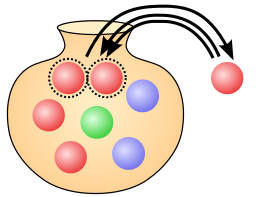
\includegraphics[scale=0.1]{../../Figures/poly_urn.png}
\begin{itemize}
  \item Consider an urn of $N$ balls of color in $E=\{1,\ldots, p\}$
  \item Draw a ball of color $x\in E$
  \item Replace the ball together with $r$ balls of color $x$ 
\end{itemize}
$p$ is the number of peers and $r$ is the size of the block reward. 
\end{column}
\end{columns}
\begin{tcolorbox}[enhanced,drop shadow, title=Theorem]
The proportion of coins owned by each peer is stable on average over the long run
\end{tcolorbox}

\tiny
\begin{thebibliography}{1}

\bibitem{Rosu2021}
I.~Ro{\c{s}}u and F.~Saleh, ``Evolution of shares in a proof-of-stake
  cryptocurrency,'' {\em Management Science}, vol.~67, pp.~661--672, feb 2021.
  \end{thebibliography}
\end{frame}

\end{document}
